\documentclass[9pt,twocolumn,twoside]{../../styles/osajnl}
\usepackage{fancyvrb}
\journal{i524} 

\title{Dryad : Distributed Execution Engine}

\author[1]{Shahidhya Ramachandran}

\affil[1]{School of Informatics and Computing, Bloomington, IN 47408, U.S.A.}

\affil[*]{Corresponding authors: shahrama@iu.edu}

\dates{Technology paper 2, \today}

\ociscodes{Dryad, Distribute Processing, Concurrent Processing, Dryad LINQ, Dataflow, Cluster Computing}

% replace this with your url in github/gitlab
\doi{\url{https://github.com/shah0112/sp17-i524/paper2/S17-IR-2027/report.pdf}}

\begin{abstract}
Dryad is a general purpose execution environment for distributed, data parallel applications and it automatically handles job creation and management, resource management, job monitoring and visualization, fault tolerance, re-execution, scheduling, and accounting. It creates a dataflow graph by using computational 'vertices' and communication 'channels'. Dryad is the middleware abstraction that is independent of the semantics of the program. It is not suitable for real-time processing since it focuses on throughput rather than latency. \newline
\end{abstract}

\setboolean{displaycopyright}{true}

\begin{document}
\maketitle

\section{Introduction}
With the expansion of the large scale Internet services that depend on clusters of thousands of servers it became more complicated to manage wide-area distributed computing. Some of the prominent challenges included high-latency, unreliable networks, control of resources by separate federated or competing entities, and issues of identity for authentication and access control \cite{DryadMSR1}. Dryad was launched in an effort to make it easier for developers to write efficient parallel and distributed applications without having in-depth knowledge of concurrent programming \cite{www-Dryad1} It focused primarily on reliability, efficiency and scalability of the applications.
Dryad was launched as a research project at MSR(Microsoft Research) and was released in EuroSys’07, March 21–23, 2007, Lisboa, Portugal \cite{DryadMSR}.\\
A Dryad application is a graph generator which can synthesize any given directed acyclic graph. These graphs are dynamic and can change depending on computations made during run-time \cite{www-Dryad1}. The vertices of the Directed Acyclic Graph define the operations that are to be performed on the data. These 'computational vertices' are written as single threaded sequential C++ constructs and are connected using one-way channels. Channels facilitate communication between the  vertices through temporary files, TCP/IP streams, and shared-memory FIFOs \cite{DryadMSR1}. The graph is parallelized by distributing the vertices across multiple execution engines. Dryad can scale this across multiple processor cores on the same computer or different physical computers connected by a network, as in a cluster \cite{DryadMSR1}. Scheduling of the computational vertices on the available hardware is handled by the Dryad run-time, without any explicit intervention by the developer of the application or administrator of the network.

\section{Dryad System}
A Dryad job is a directed acyclic graph where each vertex is a program and edges represent data channels. The logical computation graph is automatically mapped onto physical resources by run-time. The number of vertices in the graph can be much greater than the number of execution cores in the computing cluster. During run-time a finite sequence of 'structured items' are transported through the channels. channels produce and consume heap objects that inherit from a base type. The vertex program then reads and writes its data in the same way irrespective of how the channel serializes its data. Each application has its own serialization/deserialization routine \cite{DryadMSR2}.
\begin{figure}[htbp]
\begin{center}
\centering
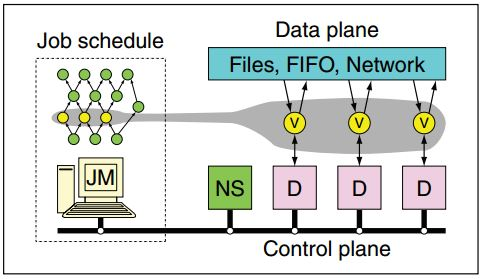
\includegraphics[width=\linewidth]{images/img1}
\caption{The Dryad system organization Source:\cite{DryadMSR2}}
\label{fig:false-color}
\end{center}
\end{figure}\\
The overall structure of a Dryad system is shown in the Figure 1. The job manager (JM) consults the name server (NS) to discover the list of available computers. It maintains the job graph and schedules running vertices (V) as computers become available using the daemon (D) as a proxy. Vertices exchange data through files, TCP pipes, or shared-memory channels. The shaded bar indicates the vertices in the job that are currently running \cite{DryadMSR2}. 
\subsection{Job Manager(JM)}
A Dryad job is coordinated by the job manager. It runs either within the cluster or on a user’s workstation with network access to the cluster. It contains the code to construct the communication graph and also the library code to schedule the work across the available resources. Job manager handles only the control decisions and is not involved in the actual data transfer between vertices \cite{DryadMSR2}
\subsection{Name Server(NS)} 
The Name Server lists all the available computers and exposes the position of each computer within the network topology so that scheduling decisions can be taken by taking locality into consideration \cite{DryadMSR2}
\subsection{Daemon(D)}
It is a cluster that runs on each of the computers and is responsible for creating processes on behalf of the job manager. The first time a vertex (V) is executed its binary is sent from the job manager to the daemon. It acts as a proxy to the job manager when it checks the status of the computation and how much data has been read and written on the channels of the remote vertices \cite{DryadMSR2}
\subsection{Job Scheduler}
The task scheduler is used to queue batch jobs. A distributed storage system is used that allows large files to be broken into small pieces, replicated and distributed across the local disks of the cluster computers \cite{DryadMSR2}
\section{Dryad Graph}
Each graph is represented as $G = <V_G, E_G, I_G, O_G>$ \cite{DryadMSR2} where $V_G$ is a   sequence of vertices with $E_G$ directed edges and two sets $I_G \subset V_G$ and  $O_G \subset V_G$ indicate the input and output vertices respectively. Directed Acyclic graphs are used because a vertex can run anywhere once its inputs have been received, it does not lead to a dead-lock situation and the finite length channels ensure that the process will definitely terminate \cite{www-DryadYT}. Figure 2 shows an example of a Directed Acyclic Graph. One of the primary restrictions on a Dryad job is that it has to be representable as a Directed Acyclic Graph. The graph can have multiple edges between the vertices. Each circle represents a program that processes a set of inputs and outputs the results. The inputs and outputs in the graph are virtual vertices of the distributed Dryad system. 
\begin{figure}[htbp]
\begin{center}
\centering
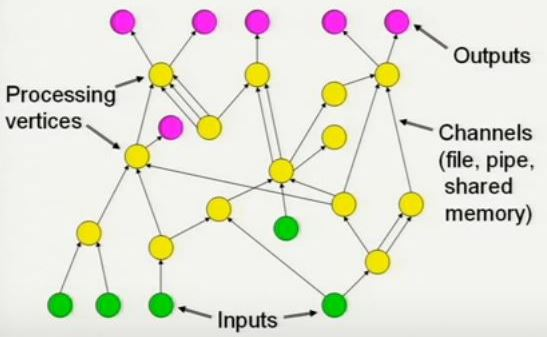
\includegraphics[width=\linewidth]{images/img2}
\caption{Directed Acyclic Graph in Dryad job Source:\cite{www-DryadYT}}
\label{fig:false-color}
\end{center}
\end{figure}
\subsection{Inputs and Outputs}
Large input files are partitioned and distributed
across the computers of the cluster. The input is grouped into a graph $G = V_P , \phi, \phi, V_P$ where $V_P$ \cite{DryadMSR3} is a sequence of virtual vertices corresponding to the partitions of the input. After the job is completed, a set of output partitions are concatenated to form a single named distributed file. An application will generally interrogate its input graphs to read the number of partitions at run-time and automatically generate the appropriately replicated graph.
\subsection{Creating new vertices}
All vertex programs inherit from the Dryad defined C++ base class. Each program has a textual name - unique within the application and a static factory- that has knowledge of constructing it \cite{DryadMSR3}. A graph vertex is created by calling the appropriate static program factory. Vertex specific parameters are set by calling methods on the program object. These parameters along with the unique vertex name form a closure that is sent to a remote process for execution.
\subsection{Adding graph edges}
New edges are created by applying a composition operation to two existing graphs as shown in Figure 3. In this figure, Circles are vertices and arrows are graph edges. A triangle at the bottom of a vertex indicates an input and one at the top indicates an output. Boxes (a) and (b) demonstrate cloning individual vertices using the carat operator. The two standard connection operations are pointwise composition using >= shown in (c) and complete bipartite composition using >> shown in (d). (e) illustrates a merge using ||. The second line of the figure shows more complex patterns. The merge in (g) makes use of a “subroutine” from (f) and demonstrates a bypass operation. For example, each A vertex might output a summary of its input to C which aggregates them and forwards the global statistics to every B. Together the B vertices can then distribute the original dataset (received from A) into balanced partitions. An asymmetric fork/join is shown in (h) \cite{DryadMSR3}.
\begin{figure*}[htbp]
\begin{center}
\centering
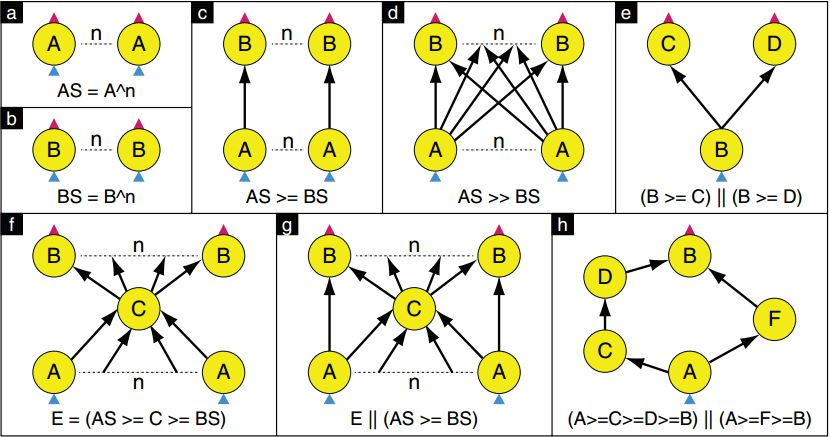
\includegraphics[width=\linewidth]{images/img3}
\caption{The operators of the graph description language Source:\cite{DryadMSR3}}
\label{fig:false-color}
\end{center}
\end{figure*}
\section{Features}
The primary features of Dryad are fault tolerance and dynamic modification of graph during run-time. \subsection{Fault Tolerance}
When a vertex execution fails, the job manager will be notified. If the vertex reported an error cleanly/crashes then it is forwarded by the daemon to the job manager. If the daemon also fails then job manager receives a heartbeat timeout. The failed vertex A is re-executed. If vertex A's inputs fail, all upstream vertices are re-executed. vertex A is running slower than it's peers then creates duplicate executions and first output is used \cite{www-DryadYT}.
\subsection{Dynamic Graph Refinement}
The application passes the initial graph at the beginning and records all the callbacks. The graphs can be modified during run-time based on the output of the computations. However, there are some restrictions that do not allow to delete a vertex once it has been executed or alter the number and type of channels \cite{www-DryadYT}. 
\section{Use cases}
Dryad can be used for any large scale computational applications, Scientific applications, Large-data processing applications- indexing, search,etc. High-level language compilers use Dryad as a run-time. For example, SCOPE (Structured Computations Optimized for Parallel Execution) and DryadLINQ \cite{www-DryadWiki}. Professor of informatics at Indiana University, Geoffrey Fox had used Dryad and DryadLINQ to analyze RADAR data focused on glaciers to earn more about the earth’s past and its present in order to make more informed, potentially life-saving predictions about its future \cite{www-DryadUse}.
\section{Performance}
\begin{figure}[htbp]
\begin{center}
\centering
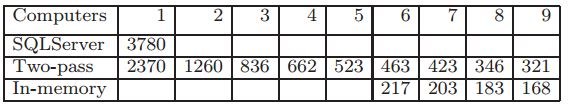
\includegraphics[width=\linewidth]{images/img4}
\caption{Time taken to process SQL query Source:\cite{DryadMSR4}}
\label{fig:false-color}
\end{center}
\end{figure}
The performance of Dryad was experimentally evaluated through two processes. In the first a relatively simple SQL query was distributed among 10 computers in the Dryad system and it performance was compared with that of a traditional commercial SQL server. The second is a map-reduce data-mining operation applied to 10.2 TBytes of data using a cluster of around 1800 computers \cite{DryadMSR4}. The experiments were run in Microsoft Research laboratory with computers having 2 dual-core Opteron processors running at 2 GHz, 8 GB of DRAM and 4 disks(400 GB). Network connectivity was by 1 Gbit/sec Ethernet links connecting into a single non-blocking switch. Figure 3 summarizes the time in seconds to process an SQL query using different numbers of computers \cite{DryadMSR4}.
\begin{figure}[htbp]
\begin{center}
\centering
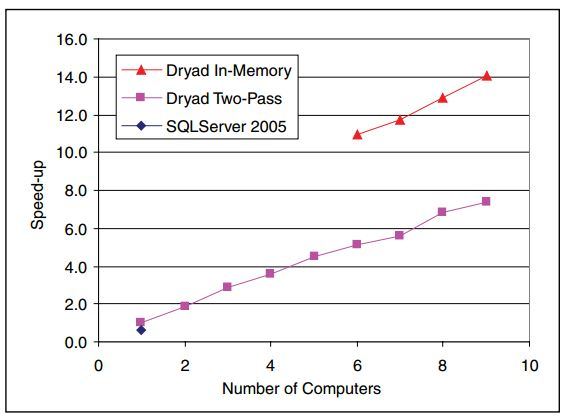
\includegraphics[width=\linewidth]{images/img5}
\caption{speedup of the SQL query Source:\cite{DryadMSR4}}
\label{fig:false-color}
\end{center}
\end{figure}
\\From Figure 5 we can see that the speedup of the SQL query computation is nearly linear in the number of computers used. The baseline is relative to Dryad running on a single computer and times are as given in Figure 4 \cite{DryadMSR4}.

\section{Conclusion}
Microsoft Dryad are suitable only for applications that take the form of a directed acyclic graph. Dryad assumes that the vertices are deterministic and will fail if the application contains non-deterministic vertices. Since the job manager assumes that it has exclusive control over the computers in the cluster, it is difficult to efficiently run more than one job at a time Dryad \cite{DryadMSR4}. It focuses only on throughput and does not improve the latency. In November 2012, Microsoft shifted their focus to Hadoop rather than improvising.  
\bibliography{references}

\end{document}
